\section{Background}\label{sec:background}

This section fixes notation and collects the results from the literature that are used later. Results
of~\cite{HHK2} are cited by their numbering in arXiv:1501.00028v1. We use $\SU$ as the group of unit
quaternions, so that a traceless element is a purely imaginary unit quaternion. Coefficients are in $\F_2$
unless stated otherwise.

\subsection{The pillowcase}\label{ss:pillowcase}
Let $G\cong\Z^2\rtimes\Z/2$ be the group of isometries of $\R^2$ generated by
$(\gamma,\theta)\mapsto(\gamma+2\pi,\theta)$, $(\gamma,\theta)\mapsto(\gamma,\theta+2\pi)$ and
$(\gamma,\theta)\mapsto(-\gamma,-\theta)$. The \emph{pillowcase} is the quotient $P=\R^2/G$, a topological
$2$-sphere. The quotient map $\R^2\to P$ is a branched covering, branched over the images of the lattice points
$(\pi\Z)^2$, which are the four \emph{corners} of $P$~\cite[\S3.1]{HHK2}. The rectangle $[0,\pi]\times[0,2\pi]$ is
a fundamental domain; we call $[0,\pi]\times[0,\pi]$ the front face, $[0,\pi]\times[\pi,2\pi]$ the back face, and
the images of the lines $\gamma\in\pi\Z$ the left and right edges. Put $\Pst=(\R^2\setminus(\pi\Z)^2)/G$, oriented
by $d\gamma\wedge d\theta$. The restriction $\R^2\setminus(\pi\Z)^2\to\Pst$ is a regular covering with deck group
$G$, so paths, loops and immersed discs in $\Pst$ lift to $\R^2\setminus(\pi\Z)^2$; we work with such lifts
throughout. The double cover $\R^2/(2\pi\Z)^2$ of $P$ is a torus, and $P$ is its quotient by the elliptic
involution $\rho(\gamma,\theta)=(-\gamma,-\theta)$.

The pillowcase is the traceless character variety of the four-punctured sphere: the space of conjugacy
classes of $\SU$ representations of $\pi_1(S^2\setminus\{a,b,c,d\})$ sending each of $a,b,c,d$ to a traceless
element is homeomorphic to $P$, and the corners correspond to the abelian
representations~\cite[Prop.~3.1]{HHK1},~\cite[Prop.~6.1]{HHK2}. We use the coordinates of Smith
(\S\ref{ss:smith-chart}) throughout.

Let $K\subset S^3$ be a knot, cut along a Conway sphere into two $2$-tangles. Restricting the traceless
representations of each tangle to the four-punctured sphere, after a holonomy perturbation, gives an immersed
curve in the pillowcase for each tangle, its perturbed traceless character variety, which may have several
components. One tangle carries the \emph{earring}, the small meridional circle that Kronheimer and Mrowka add to
the knot to define the reduced theory~\cite{KM2}, and its curve is a figure-eight curve~\cite{HHK2,HK}. Hedden,
Herald and Kirk define the Lagrangian Floer homology over $\F_2$ of the two curves and conjecture that for a
suitable decomposition it is isomorphic to the reduced singular instanton homology
$\Inat(K;\F_2)$~\cite[Conj.~6.5]{HHK2}. For an arbitrary decomposition the Floer differential is deformed by
figure-eight bubbles at the self-intersections of the curves, and Cazassus, Herald, Kirk and Kotelskiy
conjecture that each tangle, including the one that carries the earring, is assigned its perturbed character
variety together with a bounding cochain, and that the Floer homology of the two deformed curves recovers
$\Inat(K)$~\cite[Conj.~D]{CHKK}. In the algebraic model of \S\ref{ss:kwz} the assigned objects are considered up to
homotopy equivalence.

\subsection{Smith's coordinates and the sign of the perturbation}\label{ss:smith-chart}
We use the coordinates of Smith~\cite[\S2.4]{Smith}, in which the
boundary meridians satisfy $ac^{-1}=bd^{-1}$ and are sent to
\begin{equation}\label{eq:smith-coords}
a\mapsto\mathbf i,\qquad b\mapsto e^{\gamma\mathbf k}\mathbf i,\qquad c\mapsto e^{\theta\mathbf k}\mathbf i,\qquad
d\mapsto e^{(\gamma+\theta)\mathbf k}\mathbf i .
\end{equation}
The letters $a,b,c,d$, and $x,y$ in Remark~\ref{rem:sign}, denote meridians in Smith's parametrization; we
use them in this sense only in \S\ref{ss:pillowcase}, here, in Remark~\ref{rem:sign} and in the proof of
Proposition~\ref{prop:partial-triple}. Elsewhere $b$ denotes a Maurer--Cartan element and $c$ the simple
closed curve of \S\ref{ss:kh-structure}.

In these coordinates, for an appropriate holonomy perturbation, no perturbed tangle character variety meets the
corner $(\pi,\pi)$. This is~\cite[Prop.~11.1]{CHKK}, which is stated in coordinates in which the excluded corner is
$[\gamma,\theta]=[0,\pi]$; the explicit curves of Sections~\ref{sec:smith} and~\ref{sec:khovanov} miss $(\pi,\pi)$
by inspection (\S\ref{ss:explicit}). Its proof applies verbatim: an abelian traceless representation is determined by how
the tangle joins the four boundary points, and in Smith's coordinates the three possible joinings give the corner
pairs $\{(0,0),(0,\pi)\}$, $\{(0,0),(\pi,0)\}$ and $\{(\pi,0),(0,\pi)\}$. We write $Q_r$ for the rational tangle
whose traceless character variety is the straight interval of slope $r$~\cite[Prop.~2.27]{Smith}. For $r=m/n$ in
lowest terms, the line of $Q_r$ joins $(\pi,0)$ to $(0,\pi)$ if $m$ and $n$ are odd, $(0,0)$ to $(0,\pi)$ if $n$ is
even, and $(0,0)$ to $(\pi,0)$ if $m$ is even.

For tangles $T_1,T_2$ with character varieties in the pillowcase, Smith describes the character variety of the
Conway sum $T_1+T_2$ as a fiber product over $\gamma$: the $\theta$-coordinates add, and over each \emph{edge}
$\gamma\in\{0,\pi\}$ a circle of representations appears when both summands are non-abelian
there~\cite[Thms.~3.15 and~3.26]{Smith}. Smith calls such a circle \emph{internal} when it misses the
corners, and a \emph{corner circle} otherwise~\cite[Def.~3.24]{Smith}. He perturbs the sum by a holonomy
perturbation in a three-boundary configuration $C_3$: the summands are glued along two inner boundary spheres,
with pillowcases $P_1$ and $P_2$, and the sum is read off on the outer sphere, with pillowcase $P_3$. The
perturbation depends on a real parameter $t$. For small $t>0$, after an arbitrarily small additional
perturbation where needed, each internal circle is replaced by two arcs crossing once, joined crosswise to the
rest of the curve~\cite[Thm.~4.22; the crossing is drawn in Figs.~3b and~23c]{Smith}; we call this replacement the \emph{cross-resolution} of
the circle. By the symmetry described next the same holds for small $t<0$ (Proposition~\ref{prop:smith-main}).
We write $\Rp_t(T_1+T_2)$ for the perturbed character variety of the sum, mapped to $P_3$.

The two signs of $t$ give different curves. For odd $q$, a symmetry of Smith's equations maps
$\Rp_t(Q_{1/3}+Q_{1/q})$ homeomorphically onto $\Rp_{-t}(Q_{1/3}+Q_{1/q})$ and acts on $P_3$ by the
translation $(\gamma,\theta)\mapsto(\gamma+\pi,\theta)$ (Remark~\ref{rem:sign}). This translation permutes
the corners, and pairing dimensions with a fixed curve can change under it.
\emph{Throughout, $\Rp_t(Q_{1/3}+Q_{1/q})$ denotes Smith's perturbed curve for small $t<0$, and every pairing
dimension computed in Sections~\ref{sec:smith} and~\ref{sec:khovanov} is computed with this curve.}
Remarks~\ref{rem:sign-pairings} and~\ref{rem:sign-positive} record what changes for $t>0$.

\subsection{Twisted complexes over the algebra \texorpdfstring{$\mathcal B$}{B}}\label{ss:kwz}
Since tangle character varieties miss one corner, Cazassus, Herald, Kirk and Kotelskiy study them in the wrapped
Fukaya category of the pillowcase with its four corners removed, restricted to curves that do not end at that corner,
and generate the relevant subcategory by two arcs $a^\circ$, $a^\bullet$ ending at the other
corners~\cite[\S11.5]{CHKK}. The endomorphism algebra of
$a^\circ\oplus a^\bullet$ is modelled by the algebra $\mathcal B$ of Kotelskiy, Watson and
Zibrowius~\cite{KWZ}, an associative algebra whose two idempotents $\iota_\circ$ and $\iota_\bullet$
correspond to $a^\circ$ and $a^\bullet$.

To encode curves we use, following~\cite{KWZ}, the dual pair of arcs $s^\circ$, $s^\bullet$ in the chart obtained
by sending a distinguished corner to infinity (Figure~\ref{fig:chart}). Both are properly embedded with both ends
at the puncture at infinity, and we call their union the \emph{arc system}. Its complement has three faces, each
containing one of the remaining corners, and we write $L,M,R$ for the length-one paths that cross them. A positive
path is a word $X^k$ with $X\in\{L,M,R\}$ and $k\ge1$, and we write $i\xrightarrow{X^k}j$ for a matrix entry from
generator $i$ to generator $j$ labelled by $X^k$. Same-face words compose by $X^mX^n=X^{m+n}$, products of words with
two different face labels vanish, and the idempotents are units; the relations $DS=SD=0$ of the quiver
presentation of $\mathcal B$ are built into this notation. In that presentation~\cite[Def.~4.19]{KWZ}, the words
$L^k$ and $R^k$ are the powers of the loops $D$ at the two vertices and the words $M^k$ are the paths of length $k$
in the two arrows $S$, as in the decomposition of $\mathcal B$ into one cyclic quiver for each
face~\cite[Exs.~5.5 and~5.6]{KWZ}. The words $L^k$ and $R^k$ join generators of equal
idempotent, and $M^k$ joins generators of different idempotents exactly when $k$ is odd. The algebra $\mathcal B$ is
bigraded~\cite{KWZ}. We ignore the gradings, as in the comparison in~\cite[\S11.5]{CHKK}, except in
Section~\ref{sec:khovanov}, where bigradings, with $(\pi,\pi)$ as the special puncture, enter as a hypothesis of~\cite[Thm.~5.25]{KWZ}, and in the observations of \S\ref{ss:smoothings}, Remark~\ref{rem:q7-scope} and \S\ref{ss:disc-open}, which no proof uses.

\begin{figure}[ht]
\centering
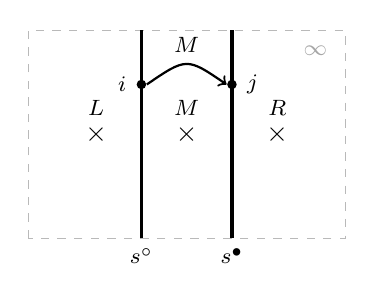
\begin{tikzpicture}[scale=1.15]
\draw[gray!55,dashed] (-1.75,-1.15) rectangle (1.75,1.15);
\draw[very thick] (-0.5,-1.15) -- (-0.5,1.15);
\draw[very thick] ( 0.5,-1.15) -- ( 0.5,1.15);
\node[below] at (-0.5,-1.15) {\footnotesize $s^{\circ}$};
\node[below] at ( 0.5,-1.15) {\footnotesize $s^{\bullet}$};
\foreach \x in {-1,0,1}{\node at (\x,0) {$\times$};}
\node[above] at (-1,0.10) {\footnotesize $L$};
\node[above] at ( 0,0.10) {\footnotesize $M$};
\node[above] at ( 1,0.10) {\footnotesize $R$};
\fill (-0.5,0.55) circle (1.5pt);  \node[left]  at (-0.56,0.55) {\footnotesize $i$};
\fill ( 0.5,0.55) circle (1.5pt);  \node[right] at ( 0.56,0.55) {\footnotesize $j$};
\draw[->,thick] (-0.44,0.55) .. controls (0,0.85) .. (0.44,0.55);
\node[above] at (0,0.80) {\footnotesize $M$};
\node[gray!70] at (1.42,0.92) {\footnotesize $\infty$};
\end{tikzpicture}
\medskip
\caption{The chart for the algebra $\mathcal B$. A distinguished corner of the pillowcase is sent to infinity,
leaving the other three corners ($\times$) in the plane. The arcs $s^{\circ},s^{\bullet}$ of the arc system cut the
chart into three faces, one for each remaining corner, labelled $L$, $M$ and $R$. In the chart used throughout
(\S\ref{ss:explicit}) the corner at infinity is $(0,\pi)$, and the faces $L$, $M$ and $R$ contain the corners
$(\pi,\pi)$, $(\pi,0)$ and $(0,0)$; Section~\ref{sec:khovanov} compares with the invariants of~\cite{KWZ} in the
normalization in which $(\pi,\pi)$ is the special puncture (\S\ref{ss:kh-smith}). A generator is an intersection
of a curve with $s^{\circ}$ or $s^{\bullet}$ and carries the idempotent $\iota_\circ$ or $\iota_\bullet$; a segment
running from $i$ to $j$ through the face $X$ contributes an arrow $i\xrightarrow{X^{k}}j$, where $k$ counts the
crossings of the arcs. Each of the faces $L$ and $R$ is bounded by a single arc of the system, so their words
join generators of equal idempotent; the face $M$ is bounded by both arcs.}
\label{fig:chart}
\end{figure}

An immersed curve in the chart that misses the corners determines an object of the category
$\operatorname{Tw}(\mathcal B)$ of twisted complexes in the standard way~\cite{KWZ}: its intersections with the arc
system are the generators, each carrying $\iota_\circ$ or $\iota_\bullet$ according to the arc it meets, and a
segment of the curve running from one intersection to the next through the face $X$ contributes the arrow
labelled by the corresponding power of $X$. Each pillowcase intersection has two lifts to the torus double cover,
interchanged by the elliptic involution $\rho$, so intersection counts on the torus are twice those on the
pillowcase.

A finite twisted complex is a finite idempotent module $V$ with a matrix $\delta$ over $\mathcal B$ satisfying
$\delta^2=0$; it is a type~D structure over $\mathcal B$ in the sense of~\cite{KWZ}, and we use the two descriptions
interchangeably. An entry of $\delta$ labelled by an idempotent is a unit, and Gaussian elimination along it
deletes its source and its target without changing the homotopy type; we call this a \emph{unit cancellation}. A
twisted complex is \emph{reduced} if every entry of $\delta$ is a sum of positive words. Two reduced twisted
complexes are \emph{strictly isomorphic} if an idempotent-preserving bijection of their generators carries one
differential to the other entry by entry. A reduced twisted complex is of \emph{loop type} if every generator
meets at most two arrows; each component of such a complex is then described by its \emph{word}, the sequence of
idempotents, labels and directions of its arrows read along the component, and a strict isomorphism of
loop-type complexes is decided by comparing the words of their components up to rotation and reversal.

For finite twisted complexes $X=(V_X,\delta_X)$ and $Y=(V_Y,\delta_Y)$, the morphism space
$\operatorname{Mor}(X,Y)$ consists of the matrices $f$ over $\mathcal B$ from $V_X$ to $V_Y$, with differential
$f\mapsto\delta_Yf+f\delta_X$. We write $\HF(X,Y):=H\operatorname{Mor}(X,Y)$, and we call
$\dim_{\F_2}\HF(X,Y)$, when it is finite, the \emph{pairing dimension} of $X$ with $Y$. For curves in the
position required by~\cite[Thm.~5.22]{KWZ}, Kotelskiy, Watson and Zibrowius show that
$\operatorname{Mor}(X,Y)$ is quasi-isomorphic to the Lagrangian Floer complex of the two curves, so the
pairing dimension is a Floer homology dimension. The hypotheses under which this identification is used are stated in Section~\ref{sec:khovanov}.

The endomorphism differential of $(V,\delta)$ is $D_\delta(b)=\delta b+b\delta$. A matrix $b$ over $\mathcal B$ is
a \emph{Maurer--Cartan element} for $(V,\delta)$ if
\begin{equation}\label{eq:typeD-MC}
(\delta+b)^2=D_\delta(b)+b^2=0,
\end{equation}
and then $(V,\delta+b)$ is again a twisted complex. There is no infinite series in~\eqref{eq:typeD-MC}: for a
suitable choice of Hamiltonian perturbations of the generating arcs, $\mu^1$ and all $\mu^k$ with $k\ge3$ vanish and
$\mu^2$ is concatenation of paths~\cite[\S11.5]{CHKK}. Cazassus, Herald, Kirk and Kotelskiy deduce this from
Bocklandt's description of the wrapped Fukaya category of a punctured surface~\cite[Thm.~7.6]{Bocklandt} and the
constructions of~\cite[\S3]{HKK}; the vanishing of the higher operations for a formal arc system is
in~\cite[\S3.4]{HKK}. The Maurer--Cartan elements used in Section~\ref{sec:smith} are supported near
self-intersection points of a curve, where they encode smoothings of the curve.

Kotelskiy, Watson and Zibrowius associate to a four-ended tangle $T$ in a ball type~D structures
$\widetilde{\mathrm{BN}}(T)$ and $\widetilde{\Kh}(T)$ over $\mathcal B$, invariants of $T$ up to homotopy
equivalence, with $\widetilde{\Kh}(T)$ the mapping cone of $H\cdot\mathrm{id}$ on
$\widetilde{\mathrm{BN}}(T)$~\cite[Def.~6.5]{KWZ}; both are represented by immersed curves, possibly with local
systems, in the four-punctured sphere~\cite{KWZ}. Their geometric pairing
theorem~\cite[Thm.~1.9]{KWZ} computes reduced Khovanov homology of a link $L=T_1\cup T_2$ obtained by gluing two
such tangles as
\[
\widetilde{\Kh}(L;\F_2)\cong\HF\bigl(\widetilde{\Kh}(mT_1),\widetilde{\mathrm{BN}}(T_2)\bigr),
\]
where $m$ denotes the mirror. For rational tangles these curves are the perturbed traceless character varieties,
$\widetilde{\mathrm{BN}}$ corresponding to the tangle and $\widetilde{\Kh}$ to the tangle with an
earring~\cite[\S1.8; for $\widetilde{\mathrm{BN}}$ also \S8.2, Prop.~8.3]{KWZ}, up to the identification of charts made in Section~\ref{sec:khovanov}.
Section~\ref{sec:khovanov} compares Smith's curve, with a Maurer--Cartan element, to
$\widetilde{\mathrm{BN}}(Q_{1/3}+Q_{1/q})$.

\subsection{The knots}\label{ss:knots}
For odd $q\ge3$ the pretzel knot $P(-2,3,q)$ is the numerator closure
\begin{equation}\label{eq:family}
P(-2,3,q)=\operatorname{num}\bigl(Q_{-1/2}+Q_{1/3}+Q_{1/q}\bigr)
\end{equation}
of a sum of rational tangles, in the convention of \S\ref{ss:smith-chart}; we write $K_q=P(-2,3,q)$. Its first two
members are the torus knots $P(-2,3,3)=T(3,4)$ and $P(-2,3,5)=T(3,5)$, and for $q\ge7$ it is
hyperbolic~\cite[Prop.~4.5]{WuebbenII}. Section~\ref{sec:smith} uses the decomposition~\eqref{eq:family} with the
earring on $Q_{-1/2}$. The companion paper~\cite{WuebbenII} uses a different decomposition, obtained from Hedden,
Herald and Kirk's decomposition of $T(3,5)$ by regluing, in which no bounding cochain is needed.
